\documentclass[border=7pt]{standalone}
\usepackage{fontspec,unicode-math}
\setmainfont{Noto Serif}
\setmathfont{STIXTwoMath-Regular.otf}
\usepackage{tikz}
\usetikzlibrary{arrows.meta,calc,patterns,decorations.pathreplacing,decorations.markings}
\tikzset{
  structure/.style={black,line width=.78pt,line join=round,line cap=round},
  potential/.style={black,line width=1.1pt,line join=round,line cap=round},
  level/.style={black,line width=1.04pt,line cap=butt},
  thinlevel/.style={black,line width=.66pt,line cap=butt},
  ax/.style={black,line width=.60pt,-{Latex[length=2mm,width=1.2mm]}},
  transition/.style={black,line width=.72pt,-{Latex[length=2mm,width=1.16mm]},shorten >=2pt,shorten <=2pt},
  dim/.style={black,line width=.66pt,{Latex[length=1.8mm,width=1mm]}-{Latex[length=1.8mm,width=1mm]}},
  annot/.style={font=\fontsize{11}{13}\selectfont,inner sep=1.6pt},
  panel/.style={font=\fontsize{13}{16}\selectfont\itshape,inner sep=1pt}
}
\pagestyle{empty}
\begin{document}
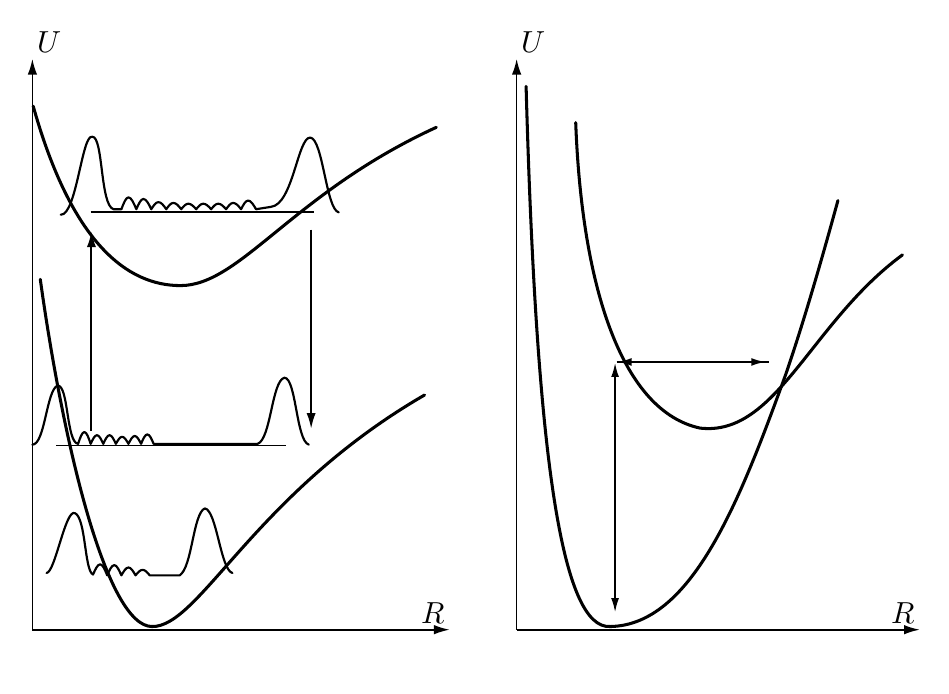
\begin{tikzpicture}[x=1cm,y=1cm]
% Source: Akulin--Karlov Fig. 19.1, printed contours traced qualitatively.
% Absolute energies and vibrational wavefunctions are not inferred experimental values.
\begin{scope}
\draw[ax] (0,0)--(5.3,0) node[annot,above left] {$R$};
\draw[ax] (0,0)--(0,7.25) node[annot,above right] {$U$};
% Potential-energy surfaces: both bound, vertically displaced minima.
\draw[potential] (.01,6.65) .. controls (.50,4.9) and (1.21,4.37) .. (1.88,4.37)
 .. controls (2.64,4.37) and (3.30,5.54) .. (5.13,6.38);
\draw[potential] (.10,4.45) .. controls (.40,2.3) and (.95,.04) .. (1.52,.04)
 .. controls (2.12,.03) and (2.82,1.73) .. (4.98,2.98);
% Vibrational wavefunctions: turning-point lobes + faint interior oscillations.
% WAVEFORM: typographic reconstruction, not a solved Schrödinger eigenfunction.
\draw[structure] (.36,5.27) .. controls (.56,5.26) and (.63,6.30) .. (.76,6.26)
 .. controls (.90,6.27) and (.86,5.39) .. (1.03,5.34)
 -- (1.13,5.34);
\draw[structure] (1.13,5.34) sin (1.22,5.49) cos (1.32,5.34)
 sin (1.41,5.47) cos (1.51,5.34) sin (1.60,5.43) cos (1.70,5.34)
 sin (1.79,5.42) cos (1.89,5.34) sin (1.98,5.41) cos (2.08,5.34)
 sin (2.17,5.41) cos (2.27,5.34) sin (2.36,5.41) cos (2.46,5.34)
 sin (2.55,5.42) cos (2.65,5.34) sin (2.74,5.45) cos (2.84,5.34)
 -- (3.03,5.37) .. controls (3.31,5.40) and (3.37,6.26) .. (3.53,6.25)
 .. controls (3.69,6.23) and (3.73,5.34) .. (3.89,5.30);
\draw[thinlevel] (.74,5.30)--(3.57,5.30);
\draw[structure] (.00,2.35) .. controls (.16,2.35) and (.18,3.05) .. (.32,3.10)
 .. controls (.46,3.11) and (.43,2.38) .. (.58,2.36)
 sin (.66,2.51) cos (.74,2.36) sin (.82,2.47) cos (.90,2.36)
 sin (.98,2.47) cos (1.06,2.36) sin (1.14,2.45) cos (1.22,2.36)
 sin (1.30,2.46) cos (1.38,2.36) sin (1.46,2.48) cos (1.54,2.36)
 -- (2.86,2.36) .. controls (3.03,2.42) and (3.04,3.16) .. (3.20,3.20)
 .. controls (3.35,3.20) and (3.35,2.40) .. (3.51,2.35);
\draw[thinlevel] (.30,2.34)--(3.22,2.34);
\draw[structure] (.18,.72) .. controls (.29,.73) and (.42,1.54) .. (.54,1.48)
 .. controls (.68,1.42) and (.66,.75) .. (.77,.70)
 sin (.86,.83) cos (.95,.69) sin (1.04,.82) cos (1.13,.69)
 sin (1.22,.79) cos (1.31,.69) sin (1.40,.76) cos (1.49,.69)
 -- (1.87,.69) .. controls (2.03,.79) and (2.04,1.48) .. (2.19,1.54)
 .. controls (2.34,1.52) and (2.39,.76) .. (2.54,.72);
% Franck--Condon: instant vertical excitation/emission at fixed R.
\draw[transition] (.75,2.45)--(.75,5.13);
\draw[transition] (3.54,5.15)--(3.54,2.48);
\node[panel] at (2.65,-.42) {а};
\end{scope}
\begin{scope}[shift={(6.15cm,0cm)}]
\draw[ax] (0,0)--(5.12,0) node[annot,above left] {$R$};
\draw[ax] (0,0)--(0,7.25) node[annot,above right] {$U$};
% Right panel: two term crossings, not a vertical radiative transition.
\draw[potential] (.12,6.9) .. controls (.25,2.20) and (.57,.0) .. (1.19,.04)
 .. controls (2.22,.06) and (2.83,1.62) .. (3.42,3.25)
 .. controls (3.65,3.92) and (3.88,4.72) .. (4.08,5.45);
\draw[potential] (.75,6.44) .. controls (.83,4.31) and (1.35,2.77) .. (2.33,2.56)
 .. controls (3.30,2.45) and (3.73,3.90) .. (4.90,4.76);
% Vertical excursion, then horizontal nuclear motion (bidirectional span).
\draw[dim] (1.25,.22)--(1.25,3.39);
\draw[dim] (1.28,3.40)--(3.16,3.40);
\draw[thinlevel] (1.27,3.40)--(3.21,3.40);
\node[panel] at (2.65,-.42) {б};
\end{scope}
\end{tikzpicture}
\end{document}
